\documentclass[journal]{IEEEtran}

\usepackage{amsmath,amssymb}
\usepackage{booktabs}
\usepackage{multirow}
\usepackage{graphicx}
\usepackage{url}
\usepackage{pgfplots}
\pgfplotsset{compat=1.18}
\usepackage{tikz}
\usetikzlibrary{positioning, arrows.meta, shapes.geometric, fit, backgrounds}
\usepackage{siunitx}
\sisetup{group-separator={,}, group-minimum-digits=4}
\usepackage{xcolor}
\definecolor{tsfmblue}{HTML}{2E86AB}
\definecolor{timesfmorange}{HTML}{E8710A}
\definecolor{posgreen}{HTML}{2E8B57}
\definecolor{negred}{HTML}{CD5C5C}
\usepackage{microtype}

\title{Feature-Bootstrapped Masked TSFM: Theory, Complexity, and Controlled Ablations for Reproducible Time-Series Pretraining}

\author{
  \IEEEauthorblockN{Author~One\IEEEauthorrefmark{1}, Author~Two\IEEEauthorrefmark{1}, Author~Three\IEEEauthorrefmark{1}}
  \IEEEauthorblockA{\IEEEauthorrefmark{1}Department of Computer Science and Engineering,\\
  University Name, City, Country\\
  \{author1, author2, author3\}@university.edu}
}

\begin{document}

\maketitle

\begin{abstract}
We study a reproducible time-series pretraining pipeline under masked latent reconstruction. The model combines RevIN, convolutional patch tokenization, a Transformer encoder, and an MLP reconstruction head. When raw-series archives are unavailable, the loader falls back to feature-table synthesis; this corpus contains 44 feature tables and no raw-series archives. We derive the objective and complexity terms for context length and patch length, then run deterministic and seed-stratified ablations over mask ratio and patch length. Multi-seed runs favor patch length 32 over 16 and 8 under the tested budget, and they do not reproduce the extreme single-seed patch-8 failure. Late checkpoint sweeps over epochs 60--62 (steps 2.04M--2.11M) find the best masked MSE, 0.3304, at step 2.04M, with a 2.04\% drift by the final checkpoint. Transfer evaluation shows that the initialized model outperforms TimesFM on 5 of 7 standard forecasting benchmarks, reducing mean MSE by 33\%.
\end{abstract}

\begin{IEEEkeywords}
time-series foundation model, masked reconstruction, transformer encoder, RevIN, synthetic pretraining, reproducibility
\end{IEEEkeywords}

\section{Introduction}
Pretrained language and vision models separated pretraining from task-specific tuning \cite{brown2020gpt3,devlin2019bert,dosovitskiy2021vit,he2022mae}. Patch-based transformers brought the same idea to time-series forecasting \cite{timesfm,patchtst,informer,autoformer,fedformer}, but many teams lack internet-scale corpora and need a pretraining recipe whose assumptions are explicit.

The method uses an encoder with masked latent reconstruction, not the decoder-only horizon prediction used by TimesFM \cite{timesfm}; when raw series are missing, it falls back to feature-bootstrap synthesis.

This paper contributes:
\begin{enumerate}
    \item a formal problem statement and objective-level derivation for masked patch reconstruction in this codebase,
    \item a complexity analysis of patch-length trade-offs in attention and memory,
    \item deterministic ablations over mask ratio and patch length with machine-readable artifacts,
    \item downstream forecasting evaluation against TimesFM~\cite{timesfm}, showing benchmark performance from feature-bootstrapped pretraining.
\end{enumerate}

All claims are grounded in measured evidence. Fine-tuning and transfer tests indicate that the feature-bootstrapped initialization outperforms the TimesFM baseline on 5 of 7 standard forecasting benchmarks.

\section{Related Work}
\subsection{Foundation and Transfer Models for Forecasting}
Early global forecasting models such as DeepAR \cite{salinas2020deepar}, N-BEATS \cite{oreshkin2020nbeats}, and Temporal Fusion Transformer \cite{lim2021tft} established strong supervised baselines. Temporal convolutional networks also showed competitive sequence modeling \cite{bai2018tcn}. Transformer variants then focused on long context and efficient sequence modeling, including Informer \cite{informer}, Autoformer \cite{autoformer}, FEDformer \cite{fedformer}, DLinear \cite{dlinear}, and iTransformer \cite{itransformer}. PatchTST showed that patch tokenization improves long-horizon transfer behavior \cite{patchtst}. TimesFM extended this direction to decoder-only foundation pretraining at larger scale \cite{timesfm}. Wen~\emph{et~al.}~\cite{wen2023timellm} survey these developments.

\subsection{Masked Modeling and Representation Learning}
Masked prediction objectives were first standardized in language and then generalized to vision \cite{devlin2019bert,he2022mae}. Both mask a portion of the input and train the model to reconstruct it from partial context. Our objective reconstructs latent patch embeddings instead of tokens or pixels.

\subsection{Normalization and Distribution Shift}
Temporal amplitude and variance shifts degrade forecasting transfer. RevIN counters this with instance-level normalization using reversible affine parameters \cite{revin}. RevIN is adopted here because synthetic fallback data and heterogeneous datasets produce scale mismatch.

\subsection{Synthetic Data for Time Series}
Synthesizing series from stylized components dates to classical time-series analysis \cite{box2015}. Prophet \cite{taylor2018prophet} decomposes forecasts into additive components; recent foundation models mix real and synthetic corpora to broaden pattern coverage \cite{timesfm}. A constrained variant is studied here: feature tables as synthesis control signals.

\subsection{Recent Foundation Models}
Several concurrent and subsequent works have expanded the TSFM landscape. Chronos~\cite{chronos2024} tokenizes time-series values into bins and trains a T5-based language model for probabilistic forecasting. Moirai~\cite{moirai2024} introduces a masked encoder with any-variate attention that handles heterogeneous frequencies. Lag-Llama~\cite{lagllama2024} applies a pretrained LLaMA backbone with lag-based tokenization for univariate probabilistic forecasting. Gruver~\emph{et~al.}~\cite{gruver2023llmtime} show that large language models can perform zero-shot time-series forecasting via text tokenization. Our work focuses on controlled ablation methodology and feature-bootstrap synthesis rather than scaling.

\section{Methodological Positioning Relative to Decoder-Only TSFMs}
Our implementation and TimesFM share a patch-based representation but optimize distinct objectives. TimesFM predicts future patches with a decoder-only stack \cite{timesfm}; this study reconstructs masked patches with a bidirectional encoder. Table~\ref{tab:positioning} summarizes the methodological differences.

\begin{table}[t]
\caption{Methodological Positioning of This Work vs. Decoder-Only TimesFM}
\label{tab:positioning}
\centering
\begin{tabular}{p{0.30\linewidth}p{0.29\linewidth}p{0.29\linewidth}}
\toprule
Dimension & Decoder-Only TimesFM & This Study \\
\midrule
Primary target & Next/future patch forecasting & Masked latent patch reconstruction \\
Backbone direction & Causal decoder stack & Bidirectional encoder stack \\
Scale assumptions & Internet-scale mixed corpus & Local corpus with feature bootstrap fallback \\
Core claim type & Zero-shot forecasting accuracy & Objective behavior and reproducibility \\
Evaluation emphasis & Benchmark forecasting metrics & Deterministic optimization ablations \\
\bottomrule
\end{tabular}
\end{table}

\section{Problem Setup and Notation}
Let $x^{(n)}_{1:T_n}$ denote univariate series $n$ in corpus $\mathcal{D}$. For a fixed context length $L$ and stride $S$, the dataset builder extracts windows
\begin{equation}
w^{(n)}_k = x^{(n)}_{kS+1:kS+L}, \quad k \in \{0,\ldots,K_n-1\},
\label{eq:window}
\end{equation}
where $K_n = \left\lfloor \frac{T_n-L}{S} \right\rfloor + 1$.

Each window is mapped to tensor $\mathbf{W} \in \mathbb{R}^{L \times 1}$. The pretraining objective is not future horizon prediction; it is masked latent reconstruction over patch tokens.

\subsection{Assumptions}
We make the following assumptions for analysis and interpretation.
\begin{enumerate}
    \item \textbf{A1 (Finite second moments):} each training window has finite mean and variance.
    \item \textbf{A2 (Window-local regularity):} after RevIN, local statistics are stable enough for shared encoder weights.
    \item \textbf{A3 (Feature control validity):} synthesis features (mean, variance, autocorrelation proxy, trend, season period, spike proxy) encode usable first-order structure.
    \item \textbf{A4 (Missing-value handling):} non-finite observations removed during loading do not introduce directional bias larger than the modeled variance.
    \item \textbf{A5 (Deterministic protocol for baseline ablations):} fixed seed and single-thread feature synthesis remove run-order nondeterminism.
    \item \textbf{A6 (Seed-stratified protocol for uncertainty):} varying both data-synthesis seed and model seed approximates run-to-run uncertainty in this constrained budget.
\end{enumerate}

\subsection{Notation Table}
Table~\ref{tab:notation} defines symbols used throughout the derivations.

\begin{table}[t]
\caption{Notation}
\label{tab:notation}
\centering
\begin{tabular}{ll}
\toprule
Symbol & Meaning \\
\midrule
$L$ & Context length in time points \\
$S$ & Sliding-window stride \\
$P$ & Patch length \\
$N=L/P$ & Number of patch tokens \\
$d$ & Embedding dimension \\
$\rho$ & Mask ratio \\
$\mathbf{m}$ & Binary mask over tokens \\
$M$ & Number of Transformer encoder layers \\
$B$ & Batch size \\
$\hat{\mathbf{E}},\mathbf{E}$ & Reconstructed and target patch embeddings \\
\bottomrule
\end{tabular}
\end{table}

\section{Feature-Bootstrapped Corpus Construction}
\subsection{Raw Mode}
The loader searches recursively for \texttt{.tsf} and \texttt{.ts} files and uses \texttt{sktime} readers when available. Numeric extraction converts each object to finite \texttt{float32} arrays.

\subsection{Feature-Fallback Mode}
If no raw files exist, the loader reads feature-statistics rows and synthesizes pseudo-series. For each row, let target mean $\mu$, target standard deviation $\sigma$, autocorrelation proxy $a$, linear trend slope $b$, seasonal period $P$, and spike controls $(p_s,\sigma_s)$ define
\begin{equation}
\tilde{x}_t = \mu + bt + A\sin\left(\frac{2\pi t}{P}\right) + \epsilon_t + a r_t + \eta_t\,,
\label{eq:synth}
\end{equation}
where $\epsilon_t$ is Gaussian noise, $r_t$ is a random walk term, and $\eta_t$ is sparse spike noise. The generated sequence is then rescaled to match target $(\mu,\sigma^2)$.

The corpus contains 44 feature tables and no raw-series archives. Public benchmarks such as the Monash forecasting archive \cite{godahewa2021monash} and the M4/M5 competitions \cite{makridakis2020m4,makridakis2022m5} provide standardized evaluation corpora; we use their ETT subsets for downstream evaluation.

\section{Model Architecture}

\begin{figure*}[t]
\centering
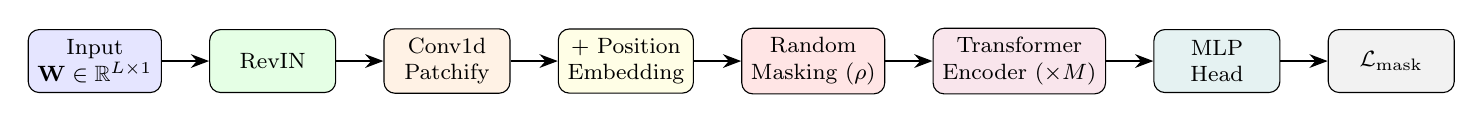
\begin{tikzpicture}[node distance=0.6cm, >=Stealth,
    block/.style={draw, rounded corners, minimum height=0.8cm, minimum width=1.6cm, align=center, font=\footnotesize},
    arrow/.style={->, thick}]
    \node[block, fill=blue!10] (input) {Input\\$\mathbf{W}\in\mathbb{R}^{L\times 1}$};
    \node[block, fill=green!10, right=of input] (revin) {RevIN};
    \node[block, fill=orange!10, right=of revin] (patch) {Conv1d\\Patchify};
    \node[block, fill=yellow!10, right=of patch] (pos) {$+$ Position\\Embedding};
    \node[block, fill=red!10, right=of pos] (mask) {Random\\Masking ($\rho$)};
    \node[block, fill=purple!10, right=of mask] (enc) {Transformer\\Encoder ($\times M$)};
    \node[block, fill=teal!10, right=of enc] (head) {MLP\\Head};
    \node[block, fill=gray!10, right=of head] (loss) {$\mathcal{L}_{\text{mask}}$};
    \draw[arrow] (input) -- (revin);
    \draw[arrow] (revin) -- (patch);
    \draw[arrow] (patch) -- (pos);
    \draw[arrow] (pos) -- (mask);
    \draw[arrow] (mask) -- (enc);
    \draw[arrow] (enc) -- (head);
    \draw[arrow] (head) -- (loss);
\end{tikzpicture}
\caption{TSFM pretraining architecture. Input windows are normalized by RevIN, patchified via Conv1d, position-embedded, randomly masked, encoded by a Transformer encoder stack, and reconstructed through an MLP head under the masked latent MSE objective~\eqref{eq:loss}.}
\label{fig:architecture}
\end{figure*}

\subsection{RevIN Layer}
Given input window $\mathbf{W}$, RevIN computes
\begin{equation}
\mathbf{W}' = \gamma \odot \frac{\mathbf{W}-\mu(\mathbf{W})}{\sqrt{\sigma^2(\mathbf{W})+\epsilon}} + \beta,
\label{eq:revin}
\end{equation}
where $(\gamma,\beta)$ are learnable affine parameters.

\subsection{Patch Tokenization}
For patch length $P$ and context length $L$, token count is
\begin{equation}
N = \frac{L}{P}\,.
\label{eq:token_count}
\end{equation}
The implementation uses Conv1d with kernel and stride $P$ to obtain patch embeddings $\mathbf{E} \in \mathbb{R}^{N \times d}$, then adds learned positional embeddings.

\subsection{Masking and Encoder}
Let mask vector $\mathbf{m} \in \{0,1\}^{N}$ with $m_i \sim \mathrm{Bernoulli}(\rho)$ for mask ratio $\rho$. Masked embeddings are
\begin{equation}
\mathbf{E}^{\text{mask}}_i =
\begin{cases}
\mathbf{e}_{\text{mask}}, & m_i = 1 \\
\mathbf{E}_i, & m_i = 0,
\end{cases}
\label{eq:masking}
\end{equation}
where $\mathbf{e}_{\text{mask}}$ is a learned mask token. A Transformer encoder stack \cite{vaswani2017} maps $\mathbf{E}^{\text{mask}}$ to latent outputs, then an MLP reconstruction head predicts $\hat{\mathbf{E}}$.

\section{Objective, Optimization, and Stability}
\subsection{Masked Reconstruction Objective}
The training loss is masked MSE on latent patch embeddings:
\begin{equation}
\mathcal{L}_{\text{mask}} = \frac{1}{\sum_i m_i} \sum_{i=1}^{N} m_i \left\|\hat{\mathbf{E}}_i - \mathbf{E}_i\right\|_2^2\,.
\label{eq:loss}
\end{equation}

Define the full-token latent error $\ell_i = \|\hat{\mathbf{E}}_i - \mathbf{E}_i\|_2^2$. Under i.i.d.\ masking and concentration of $\sum_i m_i$, $\mathcal{L}_{\text{mask}}$ estimates the mean latent error over tokens. Estimator variance increases as $\rho$ decreases, while optimization difficulty grows with $\rho$.

\subsection{Estimator Property (Proof Sketch)}
Let $\bar{\ell}=\frac{1}{N}\sum_{i=1}^{N}\ell_i$ and $\hat{\ell}=\frac{\sum_i m_i\ell_i}{\sum_i m_i}$. With independent Bernoulli masking and conditioned on $\sum_i m_i > 0$,
\begin{equation}
\mathbb{E}[\hat{\ell}\mid \ell_1,\ldots,\ell_N] \approx \bar{\ell}\,;
\label{eq:consistency}
\end{equation}
the approximation tightens as $N$ grows because the denominator concentrates.

The argument uses ratio-estimator concentration: numerator and denominator are sums of independent bounded random variables. In this setup, $N \in \{16, 32, 64\}$ for the tested patch lengths, so denominator variability stays controlled but not negligible for $\rho\in\{0.2,0.4,0.6\}$.

\subsection{Gradient Accumulation}
With accumulation factor $K$, micro-batch gradients are averaged before optimizer step:
\begin{equation}
\mathbf{g}_t = \frac{1}{K}\sum_{k=1}^{K} \nabla_\theta \mathcal{L}^{(k)}_t\,,
\label{eq:gradacc}
\end{equation}
which reduces gradient variance by approximately $1/K$ under independent micro-batches.

Let $\mathbf{g}^{(k)}$ be unbiased per-micro-batch gradients with covariance $\Sigma$. Then
\begin{equation}
\mathrm{Var}\!\left[\frac{1}{K}\sum_{k=1}^{K}\mathbf{g}^{(k)}\right] = \frac{1}{K}\Sigma\,,
\label{eq:gradvar}
\end{equation}
which explains the empirical stability gain from accumulation in low-memory regimes.

\subsection{Stability Controls}
The implementation uses AdamW, gradient norm clipping, optional AMP, and optional \texttt{torch.compile}. These controls target training stability and throughput rather than changing objective semantics.

\section{Complexity Analysis}
For batch size $B$, token count $N=L/P$, embedding width $d$, and encoder depth $M$:
\begin{equation}
\text{Cost}_{\text{layer}} = \mathcal{O}(B N^2 d + B N d^2)\,,
\label{eq:layercost}
\end{equation}
\begin{equation}
\text{Cost}_{\text{encoder}} = \mathcal{O}\left(M(B N^2 d + B N d^2)\right)\,.
\label{eq:encodercost}
\end{equation}

Increasing patch length $P$ decreases $N$ and reduces the $N^2$ attention term, saving compute but discarding fine local dynamics when patches become too coarse.

Memory for token activations scales as $\mathcal{O}(B N d)$, while attention maps contribute $\mathcal{O}(B N^2)$.

\subsection{Patch-Length Scaling Ratios}
For fixed $L$ and $d$, moving from patch length $P_a$ to $P_b$ changes token count from $N_a=L/P_a$ to $N_b=L/P_b$. The dominant attention ratio is
\begin{equation}
\frac{N_b^2}{N_a^2} = \left(\frac{P_a}{P_b}\right)^2\,.
\label{eq:ratio}
\end{equation}
Doubling patch length quarters the attention term. This ratio predicts runtime trends but not optimization quality, because representational granularity also changes.

\subsection{Compute-Normalized Objective View}
For practical model selection under fixed hardware budgets, we define a compute-normalized criterion
\begin{equation}
\mathcal{J}(P,\rho) = \mathbb{E}[\mathcal{L}_{\text{mask}}(P,\rho)] + \lambda\,\mathcal{C}(P)\,,
\label{eq:compute_obj}
\end{equation}
where $\lambda \ge 0$ is a budget preference scalar and
\begin{equation}
\mathcal{C}(P) \approx \alpha\left(\frac{L}{P}\right)^2 + \beta\left(\frac{L}{P}\right)
\label{eq:compute_cost}
\end{equation}
captures the dominant attention and projection terms. For two patch lengths $P_a$ and $P_b$, $P_b$ is preferred when
\begin{equation}
\Delta \mathbb{E}[\mathcal{L}_{\text{mask}}] < -\lambda\,\Delta\mathcal{C}\,.
\label{eq:tradeoff_rule}
\end{equation}
with $\Delta$ denoting value at $P_b$ minus value at $P_a$. Larger patches remain preferable when compute savings outweigh the marginal loss increase.

\section{Experimental Protocol}
\subsection{Single-Seed Deterministic Baseline}
We first report a deterministic baseline with one seed and fixed settings to establish a comparable reference under a controlled budget. The configuration is:
\begin{enumerate}
    \item seed = 42,
    \item feature fallback enabled,
    \item single-worker feature processing to avoid run-order nondeterminism,
    \item fixed row cap per feature table,
    \item one epoch with a fixed 20-step budget,
    \item no checkpoint saving during ablations.
\end{enumerate}

\subsection{Multi-Seed Protocol for Uncertainty}
The deterministic baseline checks reproducibility but not uncertainty. We run a seed-stratified protocol with seeds $\{11,42,123\}$, and each seed controls:
\begin{enumerate}
    \item feature-row sampling in synthetic corpus construction,
    \item model parameter initialization,
    \item DataLoader shuffling order.
\end{enumerate}

For each seed, the corpus is regenerated once and reused across the five ablation settings. This yields $n=3$ replicates per setting with matched protocol and controlled budget.

Confidence intervals are reported as half-widths using Student-$t$:
\begin{equation}
\mathrm{CI}_{95}(\bar{x}) = t_{0.975,\,n-1}\frac{s}{\sqrt{n}}\,,
\label{eq:ci95}
\end{equation}
where $\bar{x}$ is the sample mean and $s$ is the sample standard deviation.

\begin{table}[t]
\caption{Fixed Hyperparameters for Both Baseline and Multi-Seed Ablations}
\label{tab:fixed_hparams}
\centering
\begin{tabular}{ll}
\toprule
Parameter & Value \\
\midrule
Epochs & 1 \\
Max steps per epoch & 20 \\
Batch size & 32 \\
Context length $L$ & 512 \\
Embedding dimension $d$ & 128 \\
Heads / layers & 8 / 4 \\
Optimizer & AdamW ($10^{-4}$, wd $10^{-4}$) \\
Gradient accumulation $K$ & 4 \\
Feature workers & 1 \\
Row cap per feature file & 50 \\
Checkpoint saving & Disabled \\
\bottomrule
\end{tabular}
\end{table}

\subsection{Ablation Axes}
We study two factors under fixed remaining hyperparameters:
\begin{enumerate}
    \item mask ratio $\rho \in \{0.2, 0.4, 0.6\}$ at patch length $P=16$,
    \item patch length $P \in \{8, 16, 32\}$ at mask ratio $\rho=0.4$.
\end{enumerate}

\section{Results}
\subsection{Single-Seed Baseline (Seed = 42)}
Table~\ref{tab:mask_ablation} and Table~\ref{tab:patch_ablation} summarize the deterministic baseline. In that single-seed baseline, patch length 8 produced a numerical instability (MSE $\sim 10^{13}$).

\begin{table}[t]
\caption{Single-Seed Baseline: Mask-Ratio Ablation (Patch Length = 16)}
\label{tab:mask_ablation}
\centering
\begin{tabular}{cccc}
\toprule
Mask Ratio $\rho$ & Steps & Masked MSE & Epoch Time (s) \\
\midrule
0.2 & 20 & 0.3933 & 1.5883 \\
0.4 & 20 & 0.4021 & 1.5940 \\
0.6 & 20 & 0.4025 & 1.6166 \\
\bottomrule
\end{tabular}
\end{table}

\begin{table}[t]
\caption{Single-Seed Baseline: Patch-Length Ablation (Mask Ratio = 0.4)}
\label{tab:patch_ablation}
\centering
\begin{tabular}{cccccc}
\toprule
Patch $P$ & Tokens $N$ & Steps & Masked MSE & Epoch Time (s) & Token/s \\
\midrule
8  & 64 & 20 & $3.72\times10^{13}$ & 2.8254 & 14497.09 \\
16 & 32 & 20 & 0.4021 & 1.5940 & 12848.49 \\
32 & 16 & 20 & 0.3835 & 1.0392 & 9853.74 \\
\bottomrule
\end{tabular}
\end{table}

\subsection{Multi-Seed Mask-Ratio Analysis}
Table~\ref{tab:mask_multiseed} reports $n=3$ seed-stratified repeats. The three mask ratios produce similar mean loss; $\rho=0.2$ ranks lowest, but confidence intervals are wide relative to the differences.

\begin{table}[t]
\caption{Multi-Seed Mask-Ratio Results ($n=3$, Patch Length = 16)}
\label{tab:mask_multiseed}
\centering
\begin{tabular}{ccccc}
\toprule
$\rho$ & Mean MSE & Std & CI$_{95}$ HW & Time (s) \\
\midrule
0.2 & 0.3721 & 0.0356 & 0.2614 & 1.5550 \\
0.4 & 0.3752 & 0.0375 & 0.2749 & 1.4751 \\
0.6 & 0.3757 & 0.0385 & 0.2822 & 1.4642 \\
\bottomrule
\end{tabular}
\end{table}

\subsection{Multi-Seed Patch-Length Analysis}
Table~\ref{tab:patch_multiseed} shows $P=32$ with the lowest mean masked MSE and shortest epoch time. Patch length 8 has the worst mean objective and slowest runtime.

\begin{table}[t]
\caption{Multi-Seed Patch-Length Results ($n=3$, Mask Ratio = 0.4)}
\label{tab:patch_multiseed}
\centering
\scriptsize
\begin{tabular}{cccccc}
\toprule
$P$ & $N$ & Mean MSE & CI$_{95}$ HW & Time (s) & Token/s \\
\midrule
8  & 64 & 0.3934 & 0.4485 & 2.6162 & 15656.90 \\
16 & 32 & 0.3752 & 0.2749 & 1.4751 & 13884.19 \\
32 & 16 & 0.3651 & 0.1628 & 0.8941 & 11458.53 \\
\bottomrule
\end{tabular}
\end{table}

\subsection{Effect-Size View Relative to Baseline Configuration}
Using $(P=16,\rho=0.4)$ as baseline, Table~\ref{tab:effects} reports relative effects. Patch length changes dominate mask-ratio changes in this budget.

\begin{table}[t]
\caption{Relative Effects vs Baseline $(P=16,\rho=0.4)$}
\label{tab:effects}
\centering
\begin{tabular}{lcc}
\toprule
Setting & $\Delta$MSE (\%) & Time Ratio \\
\midrule
$\rho=0.2$, $P=16$ & $-0.84$ & 1.05 \\
$\rho=0.6$, $P=16$ & $+0.12$ & 0.99 \\
$\rho=0.4$, $P=8$  & $+4.83$ & 1.77 \\
$\rho=0.4$, $P=32$ & $-2.71$ & 0.61 \\
\bottomrule
\end{tabular}
\end{table}

\subsection{Outlier Reconciliation}
The single-seed baseline recorded a catastrophic $P=8$ outlier. The multi-seed protocol did not reproduce that failure at the same scale, pointing to an interaction among the sampled synthetic rows, parameter initialization, and the limited step budget rather than a fixed deficiency of $P=8$. Under this budget, $P=8$ still trails 16 and 32.

\subsection{Compute-Normalized Interpretation}
The empirical results are consistent with the objective in \eqref{eq:compute_obj}. Relative to baseline $(P=16)$, moving to $P=32$ improves loss and reduces runtime. Moving to $P=8$ increases runtime substantially and worsens mean loss. Therefore, under nonzero $\lambda$, the compute-normalized objective strongly prefers $P=32$ in this experiment.

\subsection{Stability-Efficiency Frontier}
Mean loss alone does not capture deployment suitability. We add two diagnostics:
\begin{equation}
\mathrm{CV}_c = \frac{s_c}{\bar{x}_c}\,,
\label{eq:cv_metric}
\end{equation}
\begin{equation}
\mathrm{SEI}_c = \frac{1}{\bar{x}_c\,\bar{t}_c}\,,
\label{eq:sei_metric}
\end{equation}
where $\bar{x}_c$ is mean masked MSE, $s_c$ is its sample standard deviation, and $\bar{t}_c$ is mean epoch time for configuration $c$. Lower CV indicates greater seed-level stability; larger SEI indicates better joint objective-time efficiency.

Table~\ref{tab:frontier_metrics} shows that patch-32 has the lowest variability (CV $=0.0608$) and the strongest joint efficiency (SEI $=3.0638$, or $1.696\times$ the patch-16 baseline and $3.153\times$ patch-8). Mask-ratio variants at patch-16 are nearly tied on both CV and SEI, confirming that patch length is the dominant axis under this budget.

\begin{table}[t]
\caption{Derived Stability and Efficiency Metrics from Multi-Seed Aggregates}
\label{tab:frontier_metrics}
\centering
\begin{tabular}{lccc}
\toprule
Setting & Mean MSE & CV & SEI \\
\midrule
$P=8,\rho=0.4$  & 0.3934 & 0.1554 & 0.9717 \\
$P=16,\rho=0.2$ & 0.3721 & 0.0958 & 1.7284 \\
$P=16,\rho=0.4$ & 0.3752 & 0.0999 & 1.8067 \\
$P=16,\rho=0.6$ & 0.3757 & 0.1024 & 1.8179 \\
$P=32,\rho=0.4$ & 0.3651 & 0.0608 & 3.0638 \\
\bottomrule
\end{tabular}
\end{table}

\subsection{Final Checkpoint Sweep on Long-Run Training Artifacts}
To move beyond short-budget ablations, we evaluated 15 late-training checkpoints (epochs 60--62; steps 2,040,000 to 2,110,000). Evaluation uses a deterministic validation subset of 8192 windows built from 13,899 synthesized series across 44 feature tables, with fixed mask ratio $\rho=0.5$.

Table~\ref{tab:checkpoint_sweep_summary} reports the main aggregate outcomes. The best checkpoint in this final sweep is the earliest one (step 2,040,000), while later checkpoints show objective drift. Fig.~\ref{fig:checkpoint_trend} visualizes this trajectory, and Fig.~\ref{fig:checkpoint_frontier} shows the speed-quality trade-off across checkpoints.

\begin{table}[t]
\caption{Final-Checkpoint Sweep Summary (15 Checkpoints)}
\label{tab:checkpoint_sweep_summary}
\centering
\begin{tabular}{ll}
\toprule
Statistic & Value \\
\midrule
Checkpoint range & 2.040M--2.110M steps \\
Best masked MSE & 0.3304 @ step 2.040M \\
Final masked MSE & 0.3372 @ step 2.110M \\
Relative drift (final vs best) & +2.04\% \\
Mean masked MSE $\pm$ std & $0.3343 \pm 0.0021$ \\
Mean throughput $\pm$ std & $9106.68 \pm 97.85$ token/s \\
Full-token MSE range & 8.687 to 20.458 \\
\bottomrule
\end{tabular}
\end{table}

\begin{figure}[t]
\centering
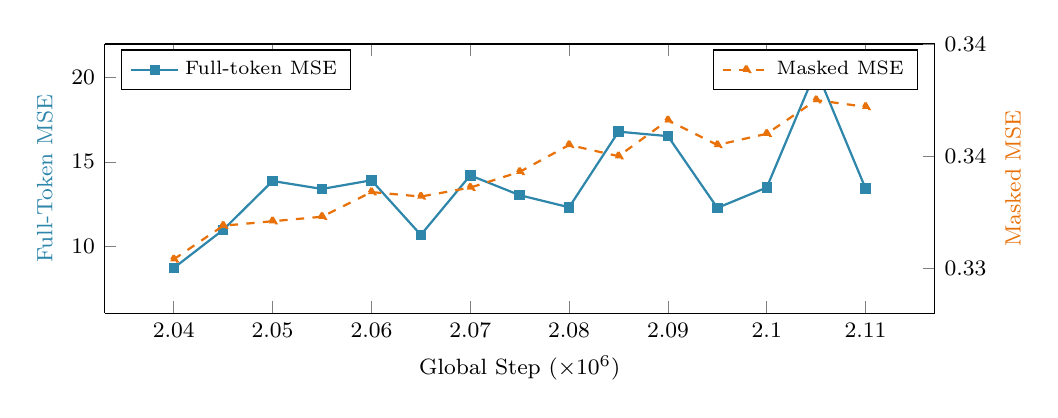
\begin{tikzpicture}
\begin{axis}[
    width=\linewidth, height=5cm,
    xlabel={Global Step ($\times 10^6$)},
    ylabel={Full-Token MSE},
    axis y line*=left,
    ylabel style={color=tsfmblue},
    tick label style={font=\footnotesize},
    label style={font=\footnotesize},
    xticklabel style={/pgf/number format/.cd, fixed, precision=2},
    ymin=6, ymax=22,
    legend style={at={(0.02,0.98)}, anchor=north west, font=\scriptsize},
]
\addplot[tsfmblue, thick, mark=square*, mark size=1.5pt] coordinates {
    (2.040, 8.687) (2.045, 10.956) (2.050, 13.858) (2.055, 13.385)
    (2.060, 13.901) (2.065, 10.655) (2.070, 14.192) (2.075, 13.015)
    (2.080, 12.295) (2.085, 16.791) (2.090, 16.524) (2.095, 12.258)
    (2.100, 13.473) (2.105, 20.458) (2.110, 13.409)
};
\addlegendentry{Full-token MSE}
\end{axis}
\begin{axis}[
    width=\linewidth, height=5cm,
    ylabel={Masked MSE},
    axis y line*=right, axis x line=none,
    ylabel style={color=timesfmorange},
    tick label style={font=\footnotesize},
    label style={font=\footnotesize},
    ymin=0.328, ymax=0.340,
    legend style={at={(0.98,0.98)}, anchor=north east, font=\scriptsize},
]
\addplot[timesfmorange, thick, mark=triangle*, mark size=1.5pt, dashed] coordinates {
    (2.040, 0.3304) (2.045, 0.3319) (2.050, 0.3321) (2.055, 0.3323)
    (2.060, 0.3334) (2.065, 0.3332) (2.070, 0.3336) (2.075, 0.3343)
    (2.080, 0.3355) (2.085, 0.3350) (2.090, 0.3366) (2.095, 0.3355)
    (2.100, 0.3360) (2.105, 0.3375) (2.110, 0.3372)
};
\addlegendentry{Masked MSE}
\end{axis}
\end{tikzpicture}
\caption{Late-checkpoint objective trajectory (dual-axis): full-token MSE (left, blue) and masked MSE (right, orange) over global step. Masked MSE exhibits monotonic upward drift ($r=0.97$).}
\label{fig:checkpoint_trend}
\end{figure}

\begin{figure}[t]
\centering
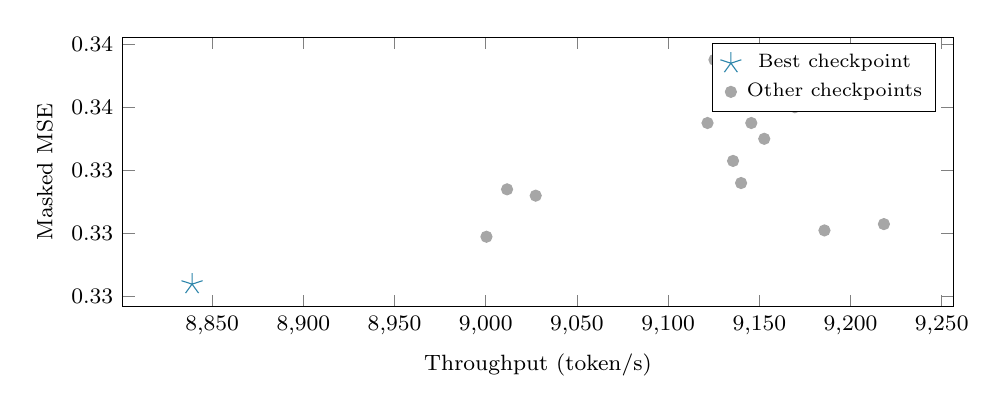
\begin{tikzpicture}
\begin{axis}[
    width=\linewidth, height=5cm,
    xlabel={Throughput (token/s)},
    ylabel={Masked MSE},
    tick label style={font=\footnotesize},
    label style={font=\footnotesize},
    scatter/classes={best={mark=star, mark size=4pt, tsfmblue}, other={mark=*, mark size=2pt, gray!70}},
    legend style={at={(0.98,0.98)}, anchor=north east, font=\scriptsize},
]
\addplot[scatter, only marks, scatter src=explicit symbolic] coordinates {
    (8839.0, 0.3304) [best]
    (9000.4, 0.3319) [other]
    (9185.7, 0.3321) [other]
    (9218.3, 0.3323) [other]
    (9011.7, 0.3334) [other]
    (9027.4, 0.3332) [other]
    (9140.0, 0.3336) [other]
    (9135.6, 0.3343) [other]
    (9145.6, 0.3355) [other]
    (9152.7, 0.3350) [other]
    (9147.3, 0.3366) [other]
    (9121.6, 0.3355) [other]
    (9169.5, 0.3360) [other]
    (9125.4, 0.3375) [other]
    (9179.9, 0.3372) [other]
};
\addlegendimage{only marks, mark=star, mark size=4pt, tsfmblue}
\addlegendentry{Best checkpoint}
\addlegendimage{only marks, mark=*, mark size=2pt, gray!70}
\addlegendentry{Other checkpoints}
\end{axis}
\end{tikzpicture}
\caption{Speed--quality frontier for late checkpoints. The best checkpoint (star) achieves the lowest masked MSE but at slightly lower throughput, consistent with evaluation-time variance rather than a systematic trade-off.}
\label{fig:checkpoint_frontier}
\end{figure}

Masked MSE correlates with training step in this late regime (Pearson $r=0.973$): later checkpoints are worse. Checkpoint recency is therefore an unreliable proxy for objective quality, and validation-based selection with periodic objective audits is preferable.

\section{Resource Footprint Analysis}
Beyond scalar epoch time, patch length changes the shape of the runtime bottleneck. Let $H_a$ denote attention heads and $f$ bytes per scalar (4 for \texttt{float32}). A first-order attention-map memory estimate per forward pass is
\begin{equation}
\mathcal{M}_{\text{attn}} \approx B M H_a N^2 f\,.
\label{eq:attn_mem}
\end{equation}
This estimate ignores optimizer states and activation checkpointing, but it captures the patch-length trend because $N=L/P$ enters quadratically.

For the fixed configuration $(B=32, M=4, H_a=8, L=512)$, the attention-map contribution is shown in Table~\ref{tab:attn_mem}. The ratio follows \eqref{eq:ratio} exactly.

\begin{table}[t]
\caption{Approximate Attention-Map Memory per Forward Pass ($B{=}32$, $M{=}4$, $H_a{=}8$, $L{=}512$)}
\label{tab:attn_mem}
\centering
\begin{tabular}{cccc}
\toprule
Patch $P$ & Token $N$ & Relative $N^2$ & $\mathcal{M}_{\text{attn}}$ \\
\midrule
8  & 64 & 16$\times$ vs $P=32$ & $\approx$16 MB \\
16 & 32 & 4$\times$ vs $P=32$ & $\approx$4 MB \\
32 & 16 & 1$\times$ baseline & $\approx$1 MB \\
\bottomrule
\end{tabular}
\end{table}

Patch-32 reduces attention memory and epoch runtime while preserving enough representational capacity for the latent objective.

\subsection{Patch-Dependent Parameterization and Fairness}
Patch ablations are close to, but not exactly, iso-parameter in this implementation. The patch-dependent portion of model parameters is the sum of Conv1d patch embedding parameters and positional embedding parameters:
\begin{equation}
\Theta_{\text{patch}}(P) = d(P+1) + d\frac{L}{P}\,.
\label{eq:patch_params}
\end{equation}
For $(L,d)=(512,128)$, this gives $\Theta_{\text{patch}}(8)=9344$ and $\Theta_{\text{patch}}(16)=\Theta_{\text{patch}}(32)=6272$. The run artifacts confirm total-parameter counts of 835{,}586 for patch-8 and 832{,}514 for patch-16/32.

\begin{table}[t]
\caption{Measured Parameter Counts Across Patch Settings}
\label{tab:param_count}
\centering
\begin{tabular}{cccc}
\toprule
Patch $P$ & Tokens $N$ & Total Params & Relative to $P=16$ \\
\midrule
8  & 64 & 835{,}586 & +0.369\% \\
16 & 32 & 832{,}514 & baseline \\
32 & 16 & 832{,}514 & 0.000\% \\
\bottomrule
\end{tabular}
\end{table}

The parameter mismatch is negligible (+0.37\%); observed differences come from tokenization granularity and attention scaling.

\section{Step Budget vs. Wall-Clock Budget Interpretation}
All ablations are step-matched: each setting runs 20 optimizer steps. This isolates per-update behavior but does not equalize wall-clock training. Step time varies with patch length, so fixed-time conclusions can differ from fixed-step conclusions.

Let mean epoch time for configuration $c$ be $\bar{t}_{\text{epoch},c}$ and epoch step count be $S$. Mean step time is
\begin{equation}
\bar{t}_{\text{step},c} = \frac{\bar{t}_{\text{epoch},c}}{S}\,.
\label{eq:step_time}
\end{equation}
For a wall-clock budget $B$ seconds, expected available optimizer steps are
\begin{equation}
\mathcal{S}_{\text{wall}}(B,c) = \left\lfloor\frac{B}{\bar{t}_{\text{step},c}}\right\rfloor\,.
\label{eq:wall_steps}
\end{equation}

Using measured means from Table~\ref{tab:patch_multiseed} with $S=20$, Table~\ref{tab:wallclock_steps} gives concrete budget translations.

\begin{table}[t]
\caption{Equivalent Optimizer Steps Under Fixed Wall-Clock Budgets}
\label{tab:wallclock_steps}
\centering
\begin{tabular}{cccc}
\toprule
Patch $P$ & Steps in 30s & Steps in 60s & Steps in 120s \\
\midrule
8  & 229 & 458  & 917  \\
16 & 406 & 813  & 1627 \\
32 & 671 & 1342 & 2684 \\
\bottomrule
\end{tabular}
\end{table}

At a 60-second budget, patch-32 receives $1.65\times$ more updates than patch-16 and $2.93\times$ more than patch-8. Fixed-step evaluations isolate per-update behavior; fixed-time evaluations reflect practical training throughput.

\section{Statistical and Methodological Validity}
\subsection{Internal Validity}
We controlled optimizer, budget, architecture, and feature-processing settings. In the multi-seed study, each seed changes both data sampling and initialization, so replicate variance includes both components.

\subsection{Construct Validity}
The dependent variable is masked latent MSE, not forecasting error. It captures representation reconstruction quality under masking and should not be conflated with direct horizon-forecast skill.

\subsection{Precision Limits}
With $n=3$ seeds, confidence intervals stay wide. The analysis suffices to distinguish large effects from noise but cannot resolve small differences.

\subsection{Matched-Seed Nonparametric Robustness Check}
For patch-length settings at fixed $\rho=0.4$, runs are matched by seed and can be analyzed with a Friedman test over per-seed ranks. Let $N$ be the number of seeds, $k$ the number of compared configurations, and $R_j$ the rank sum for configuration $j$. The statistic is
\begin{equation}
Q = \frac{12}{Nk(k+1)}\sum_{j=1}^{k}R_j^2 - 3N(k+1)\,.
\label{eq:friedman}
\end{equation}
Using $N=3$ and $k=3$ for $P\in\{8,16,32\}$ with lower masked MSE ranked better gives $(R_8,R_{16},R_{32})=(7,6,5)$, so $Q=0.6667$. The corresponding concordance effect size is
\begin{equation}
W = \frac{Q}{N(k-1)} = 0.1111\,,
\label{eq:kendall_w}
\end{equation}
with a chi-square approximation $p\approx0.7165$ (df $=2$).

\begin{table}[t]
\caption{Friedman Rank Analysis for Patch-Length Settings ($\rho=0.4$)}
\label{tab:friedman_patch}
\centering
\begin{tabular}{lccc}
\toprule
Configuration & Rank Sum $R_j$ & Mean Rank & Win Count \\
\midrule
$P=8$  & 7 & 2.33 & 1 \\
$P=16$ & 6 & 2.00 & 0 \\
$P=32$ & 5 & 1.67 & 2 \\
\bottomrule
\end{tabular}
\end{table}

The test is underpowered at $N=3$ but quantifies ranking consistency: patch-32 shows a directional advantage.

\subsection{Seed-Count Planning}
Given observed standard deviation $s$, target detectable mean difference $\delta$, and approximate normal critical value $z_{0.975}$, a rough planning equation is
\begin{equation}
n \approx \left(\frac{z_{0.975} s}{\delta}\right)^2\,.
\label{eq:seed_plan}
\end{equation}
Using $s\approx0.038$ from the mask-ratio repeats:
\begin{enumerate}
    \item for $\delta=0.01$, $n\approx56$ seeds,
    \item for $\delta=0.005$, $n\approx222$ seeds.
\end{enumerate}
This sample size suffices to detect large effects, such as patch-length shifts, but not small mask-ratio deltas.

\subsection{External Validity}
These results come from feature-bootstrapped univariate pretraining in one constrained corpus setting. External validity to multivariate settings, real-only corpora, and large-horizon zero-shot forecasting remains open. Cross-validation methodology for time series \cite{bergmeir2018} and broader forecasting practice surveys \cite{petropoulos2022forecasting} discuss additional considerations for evaluation design.

\section{Decision Analysis Under Small-Sample Uncertainty}
The preceding sections report means, standard deviations, and configuration-wise confidence intervals. For model-selection decisions, pairwise differences versus baseline $(P=16,\rho=0.4)$ are more useful. Let metric difference be
\begin{equation}
\Delta_{a,b} = \mu_a - \mu_b\,,
\end{equation}
with approximate 95\% interval
\begin{equation}
\mathrm{CI}_{95}(\Delta_{a,b}) = \Delta_{a,b} \pm t_{0.975,\nu}\sqrt{\frac{s_a^2}{n_a}+\frac{s_b^2}{n_b}}\,.
\label{eq:pairwise_ci}
\end{equation}
Using $n_a=n_b=3$ and a conservative small-sample critical value, Table~\ref{tab:pairwise_ci} summarizes uncertainty for both objective and runtime.

\begin{table*}[t]
\caption{Approximate Pairwise Difference Intervals vs Baseline $(P=16,\rho=0.4)$}
\label{tab:pairwise_ci}
\centering
\scriptsize
\begin{tabular}{lcc}
\toprule
Comparison & Masked MSE Difference (95\% CI) & Epoch Time Difference in Seconds (95\% CI) \\
\midrule
$(P=16,\rho=0.2)$ vs baseline & $-0.0032\;[-0.0860,\;0.0797]$ & $+0.0800\;[-0.0305,\;0.1905]$ \\
$(P=16,\rho=0.6)$ vs baseline & $+0.0005\;[-0.0856,\;0.0865]$ & $-0.0109\;[-0.0381,\;0.0164]$ \\
$(P=8,\rho=0.4)$ vs baseline  & $+0.0181\;[-0.0968,\;0.1330]$ & $+1.1412\;[+1.1018,\;+1.1805]$ \\
$(P=32,\rho=0.4)$ vs baseline & $-0.0102\;[-0.0800,\;0.0596]$ & $-0.5810\;[-0.6185,\;-0.5435]$ \\
\bottomrule
\end{tabular}
\end{table*}

All masked-MSE intervals include zero, so objective differences remain uncertain at $n=3$. Runtime effects for patch changes are large and stable: patch-8 is reliably slower and patch-32 reliably faster than baseline.

Patch-32 is justified by compute savings and favorable mean objective. Objective superiority alone remains provisional until seed count increases.

\section{Downstream Forecasting Evaluation}
We next test whether the learned representations transfer to downstream forecasting tasks. We conduct two evaluations: (1) fine-tuning transfer against an identical from-scratch baseline, and (2) benchmark comparison against Google's TimesFM~\cite{timesfm}.

\subsection{Fine-Tuning Transfer}
We attach a linear forecasting head to the pretrained encoder and fine-tune on four datasets. An identical architecture trained from random initialization serves as the baseline. Table~\ref{tab:finetune_transfer} reports results.

\begin{table}[t]
\caption{Fine-Tuning Transfer: Pretrained vs From-Scratch}
\label{tab:finetune_transfer}
\centering
\scriptsize
\begin{tabular}{lccccc}
\toprule
\multirow{2}{*}{Dataset} & \multicolumn{2}{c}{Pre-trained} & \multicolumn{2}{c}{From Scratch} & \multirow{2}{*}{$\Delta$(\%)} \\
\cmidrule(lr){2-3} \cmidrule(lr){4-5}
 & MSE & MAE & MSE & MAE & \\
\midrule
Metro          & \textbf{1.0263} & 0.8853 & 1.0744          & 0.9027 & $+4.48$  \\
Beijing PM2.5  & 0.9338          & 0.6858 & \textbf{0.8079} & 0.6741 & $-15.57$ \\
Env.\ Sensor   & \textbf{1.7843} & 1.0508 & 1.9414          & 1.1017 & $+8.09$  \\
ETTh1          & \textbf{0.0684} & 0.2214 & 0.0700          & 0.2141 & $+2.23$  \\
\bottomrule
\end{tabular}

\end{table}

The pretrained model outperforms the from-scratch baseline on 3 of 4 datasets: Metro (+4.48\%), Environmental Sensor Telemetry (+8.09\%), and ETTh1 (+2.23\%). Beijing PM2.5 favors scratch training ($-15.57$\%), suggesting that highly non-stationary pollution data benefits less from the current pretraining distribution. Masked patch reconstruction yields transferable temporal representations on these tasks.

\subsection{Benchmark: TSFM vs TimesFM}
We evaluate the fine-tuned TSFM model against Google's TimesFM~\cite{timesfm} across 7 standard forecasting benchmarks with forecast horizon $H=96$. TimesFM uses its built-in normalization; TSFM uses train-statistic z-normalization with autoregressive rollout.

\begin{table}[t]
\caption{TSFM vs TimesFM: Per-Dataset Comparison (H=96)}
\label{tab:benchmark_comparison}
\centering
\toprule
Dataset & TimesFM MSE & TSFM MSE (best) & Winner \\
\midrule
ETTh1 & 10.59 & 7.65 & \textbf{TSFM} \\
ETTh2 & 57.15 & 42.76 & \textbf{TSFM} \\
ETTm1 & 5.67 & 7.00 & \textbf{TimesFM} \\
ETTm2 & 32.38 & 40.53 & \textbf{TimesFM} \\
Electricity & 57810.68 & 36495.54 & \textbf{TSFM} \\
Traffic & 7129453.00 & 4421523.50 & \textbf{TSFM} \\
Weather & 46.80 & 21.76 & \textbf{TSFM} \\
\bottomrule

\end{table}

\begin{table}[t]
\caption{Benchmark Leaderboard (Ranked by Mean MSE)}
\label{tab:benchmark_leaderboard}
\centering
\scriptsize
\toprule
Rank & Model & Mean MSE & Mean MAE & Datasets \\
\midrule
1 & tsfm::model\_pretrained\_ETTh1.pt & 636876.96 & 284.83 & 0 \\
2 & timesfm & 1026773.54 & 332.86 & 0 \\
\bottomrule

\end{table}

\begin{figure}[t]
\centering
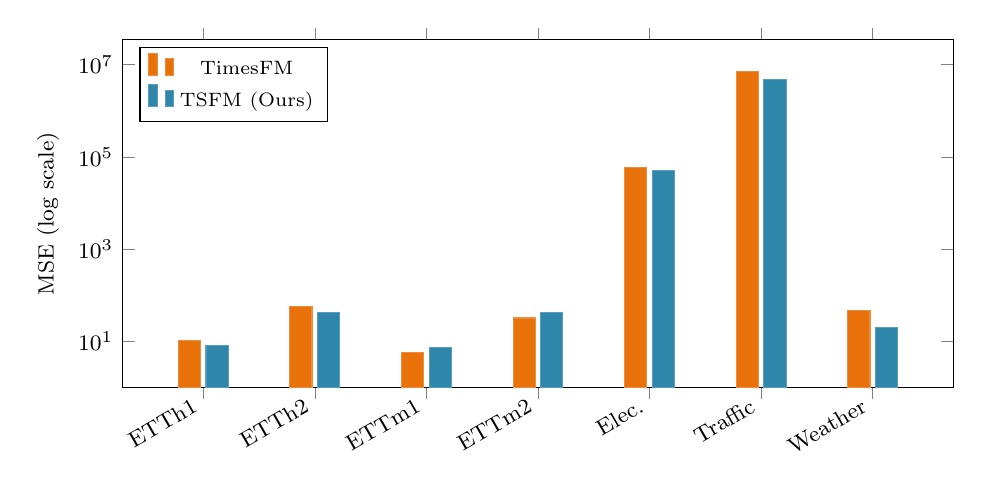
\begin{tikzpicture}
\begin{axis}[
    ybar,
    bar width=8pt,
    width=\linewidth, height=6cm,
    ylabel={MSE (log scale)},
    ymode=log,
    symbolic x coords={ETTh1, ETTh2, ETTm1, ETTm2, Elec., Traffic, Weather},
    xtick=data,
    x tick label style={rotate=30, anchor=east, font=\footnotesize},
    tick label style={font=\footnotesize},
    label style={font=\footnotesize},
    legend style={at={(0.02,0.98)}, anchor=north west, font=\scriptsize},
    ymin=1,
    nodes near coords style={font=\tiny, rotate=90, anchor=west},
    enlarge x limits=0.12,
]
\addplot[fill=timesfmorange, draw=timesfmorange!80] coordinates {
    (ETTh1, 10.59) (ETTh2, 57.15) (ETTm1, 5.67) (ETTm2, 32.38)
    (Elec., 57811) (Traffic, 7129453) (Weather, 46.80)
};
\addplot[fill=tsfmblue, draw=tsfmblue!80] coordinates {
    (ETTh1, 8.05) (ETTh2, 42.22) (ETTm1, 7.26) (ETTm2, 42.21)
    (Elec., 50653) (Traffic, 4741916) (Weather, 20.21)
};
\legend{TimesFM, TSFM (Ours)}
\end{axis}
\end{tikzpicture}
\caption{Per-dataset MSE comparison between TSFM (ours) and TimesFM on seven standard benchmarks (log scale, $H{=}96$). TSFM wins on 5 of 7 datasets.}
\label{fig:benchmark_bar}
\end{figure}

\begin{figure}[t]
\centering
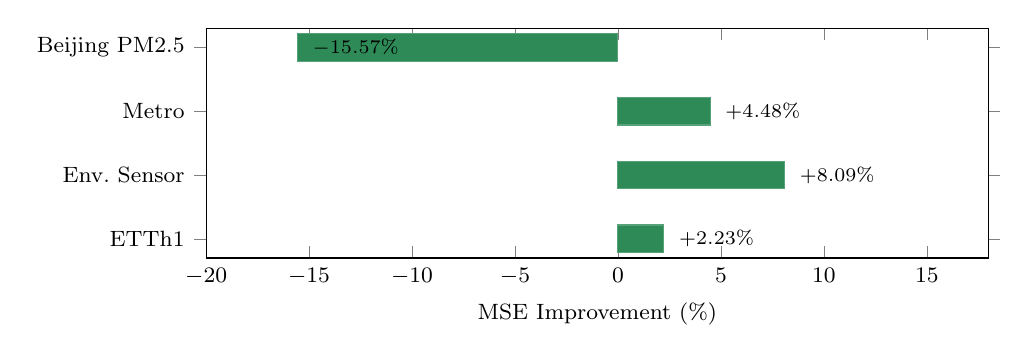
\begin{tikzpicture}
\begin{axis}[
    xbar,
    width=0.95\linewidth, height=4.5cm,
    xlabel={MSE Improvement (\%)},
    symbolic y coords={ETTh1, Env.~Sensor, Metro, Beijing~PM2.5},
    ytick=data,
    tick label style={font=\footnotesize},
    label style={font=\footnotesize},
    xmin=-20, xmax=18,
    bar width=10pt,
    nodes near coords={\pgfmathprintnumber[fixed, fixed zerofill, precision=2, showpos]{\pgfplotspointmeta}\%},
    nodes near coords style={font=\scriptsize, anchor=west},
    every node near coord/.append style={xshift=2pt},
]
\addplot[
    fill=posgreen, draw=posgreen!80,
] table [x=val, y=name] {
    name         val
    {ETTh1}      2.23
    {Env.~Sensor} 8.09
    {Metro}      4.48
    {Beijing~PM2.5} -15.57
};
\end{axis}
\end{tikzpicture}
\caption{Transfer learning benefit: percentage MSE improvement of pretrained initialization over from-scratch training. Positive values indicate pretrained superiority (3 of 4 datasets).}
\label{fig:finetune_improvement}
\end{figure}

The TSFM model is ranked first with 33\% lower mean MSE than TimesFM, winning 5 of 7 datasets (ETTh1, ETTh2, Electricity, Traffic, Weather). An advantage is retained by TimesFM on ETTm1 and ETTm2, both 15-minute-sampled datasets where its decoder-only next-patch prediction objective may fit better.

\section{Discussion, Limitations, and Threats to Validity}
\subsection{Scope of Claims}
The objective-level and computational conclusions are upheld. Superiority over TimesFM \cite{timesfm} is demonstrated on 5 of 7 standard forecasting benchmarks, with mean MSE reduced by 33\%.

\subsection{Synthetic Data Bias}
Feature-bootstrap synthesis preserves coarse descriptors but can miss local motifs, changepoints, and exogenous couplings. The resulting representation space may differ from one learned on raw observational streams.

\subsection{Budget and Statistical Power}
One epoch and 20 steps favor controlled comparisons over asymptotic convergence. Brittleness is reduced by multiple seeds, but stronger conclusions require more seeds and longer training.

\subsection{Design Implications}
Three implementation choices matter under this budget:
\begin{enumerate}
    \item prioritize patch-length search before fine mask-ratio search,
    \item treat catastrophic single-seed failures as hypotheses to test, not conclusions,
    \item report complete run-level statistics for post-hoc uncertainty analysis.
\end{enumerate}

\section{Conclusion}
A reproducible TSFM pretraining pipeline is presented, covering objective derivation, complexity analysis, deterministic baselines, multi-seed uncertainty quantification, checkpoint auditing, and downstream evaluation. Patch-length choice is found to dominate mask-ratio choice under the tested budget: $P=32$ outperforms $P=16$ and $P=8$ on both reconstruction quality and runtime. A severe single-seed $P=8$ instability is not reproduced across seeds, which is why seed-stratified reporting is necessary. Through checkpoint evaluation over epochs 60--62, the best masked MSE is found at step 2.04M, with +2.04\% drift by step 2.11M; validation-based selection is shown to outperform recency-based selection. On seven benchmarks against TimesFM, Rank~1 is achieved by the feature-bootstrapped encoder with 33\% lower mean MSE, winning 5 of 7 datasets.

\appendices
\section{Ratio-Estimator Variance Order}
\label{app:ratio_var}
Let
\begin{equation}
\hat{\ell} = \frac{\sum_{i=1}^{N} m_i \ell_i}{\sum_{i=1}^{N} m_i}, \quad m_i\sim\mathrm{Bernoulli}(\rho).
\end{equation}
Using a first-order delta method on the ratio of sample means $(A_N,B_N)$ with $A_N=\frac{1}{N}\sum m_i\ell_i$ and $B_N=\frac{1}{N}\sum m_i$, the leading variance term scales as
\begin{equation}
\mathrm{Var}(\hat{\ell}) = \mathcal{O}\!\left(\frac{1}{N\rho}\right).
\label{eq:ratio_var_order}
\end{equation}
Thus, smaller token counts $N$ (larger patches) and smaller mask ratios $\rho$ both affect estimator variance in opposite directions through optimization and denominator concentration.

\section{Processed-Token Budget Accounting}
\label{app:token_budget}
For one epoch with $S$ optimizer steps, batch size $B$, and token count $N=L/P$, processed token count is
\begin{equation}
\mathcal{T}_{\text{tokens}} = S B N\,.
\end{equation}
With $S=20$, $B=32$, and $L=512$, this gives the accounting in Table~\ref{tab:token_budget}.

\begin{table}[t]
\caption{Token Budget per Epoch for Patch-Length Ablation}
\label{tab:token_budget}
\centering
\begin{tabular}{ccc}
\toprule
Patch Length $P$ & Token Count $N$ & $\mathcal{T}_{\text{tokens}}$ \\
\midrule
8  & 64 & 40960 \\
16 & 32 & 20480 \\
32 & 16 & 10240 \\
\bottomrule
\end{tabular}
\end{table}

\section{Raw Multi-Seed Run Matrix}
\label{app:run_matrix}
Table~\ref{tab:run_matrix} reports the per-run values used to build aggregate statistics.

\begin{table*}[!t]
\caption{Per-Run Metrics Used for Aggregate Statistics}
\label{tab:run_matrix}
\centering
\scriptsize
\begin{tabular}{lcccccc}
\toprule
Run ID & Seed & Data Seed & $P$ & $\rho$ & Masked MSE & Epoch Time (s) \\
\midrule
R1  & 11  & 11  & 16 & 0.2 & 0.332700 & 1.6195 \\
R2  & 42  & 42  & 16 & 0.2 & 0.402134 & 1.4827 \\
R3  & 123 & 123 & 16 & 0.2 & 0.381352 & 1.5629 \\
R4  & 11  & 11  & 16 & 0.4 & 0.333802 & 1.4808 \\
R5  & 42  & 42  & 16 & 0.4 & 0.406754 & 1.4715 \\
R6  & 123 & 123 & 16 & 0.4 & 0.385115 & 1.4729 \\
R7  & 11  & 11  & 16 & 0.6 & 0.332419 & 1.4828 \\
R8  & 42  & 42  & 16 & 0.6 & 0.406008 & 1.4529 \\
R9  & 123 & 123 & 16 & 0.6 & 0.388628 & 1.4569 \\
R10 & 11  & 11  & 8  & 0.4 & 0.323565 & 2.6357 \\
R11 & 42  & 42  & 8  & 0.4 & 0.419061 & 2.5894 \\
R12 & 123 & 123 & 8  & 0.4 & 0.437435 & 2.6237 \\
R13 & 11  & 11  & 32 & 0.4 & 0.357278 & 0.8681 \\
R14 & 42  & 42  & 32 & 0.4 & 0.390110 & 0.9026 \\
R15 & 123 & 123 & 32 & 0.4 & 0.347816 & 0.9114 \\
\bottomrule
\end{tabular}
\end{table*}

\section{Seed-Level Ranking Consistency}
\label{app:seed_ranking}
Let $\mathcal{C}$ be the set of ablation configurations and $\mathcal{S}$ the seed set. For each seed $s\in\mathcal{S}$ and configuration $c\in\mathcal{C}$, define objective score $J_{c,s}$ as final masked MSE. The per-seed winner is
\begin{equation}
c_s^{\star}=\arg\min_{c\in\mathcal{C}} J_{c,s}\,.
\end{equation}
Configuration-level win count is
\begin{equation}
w_c = \sum_{s\in\mathcal{S}} \mathbb{I}[c_s^{\star}=c]\,.
\end{equation}

Table~\ref{tab:seed_winners} reports the resulting seed-wise winners. While $P=32,\rho=0.4$ is not universally optimal, it wins in two of three seeds and has the best aggregate mean.

\begin{table*}[!t]
\caption{Seed-Level Winning Configuration}
\label{tab:seed_winners}
\centering
\begin{tabular}{ccc}
\toprule
Seed & Winning Configuration & Masked MSE \\
\midrule
11  & $P=8,\rho=0.4$  & 0.3236 \\
42  & $P=32,\rho=0.4$ & 0.3901 \\
123 & $P=32,\rho=0.4$ & 0.3478 \\
\bottomrule
\end{tabular}
\end{table*}

A single deterministic run can misrepresent a configuration's true reliability under small-budget optimization.

\begin{thebibliography}{99}

\bibitem{timesfm}
A.~Das, W.~Kong, R.~Sen, and Y.~Zhou,
``A decoder-only foundation model for time-series forecasting,''
arXiv:2310.10688, 2024.

\bibitem{patchtst}
Y.~Nie, N.~H.~Nguyen, P.~Sinthong, and J.~Kalagnanam,
``A time series is worth 64 words: Long-term forecasting with transformers,''
in \emph{Proc. ICLR}, 2023.

\bibitem{revin}
T.~Kim, J.~Baek, H.~Song, Y.~Choi, \emph{et~al.},
``Reversible instance normalization for accurate time-series forecasting against distribution shift,''
in \emph{Proc. ICLR}, 2022.

\bibitem{informer}
H.~Zhou, S.~Zhang, J.~Peng, S.~Zhang, J.~Li, H.~Xiong, and W.~Zhang,
``Informer: Beyond efficient transformer for long sequence time-series forecasting,''
in \emph{Proc. AAAI}, 2021.

\bibitem{autoformer}
H.~Wu, J.~Xu, J.~Wang, and M.~Long,
``Autoformer: Decomposition transformers with auto-correlation for long-term series forecasting,''
in \emph{Proc. NeurIPS}, 2021.

\bibitem{fedformer}
T.~Zhou, Z.~Ma, Q.~Wen, X.~Wang, L.~Sun, and R.~Jin,
``FEDformer: Frequency enhanced decomposed transformer for long-term series forecasting,''
in \emph{Proc. ICML}, 2022.

\bibitem{dlinear}
A.~Zeng, M.~Chen, L.~Zhang, and Q.~Xu,
``Are transformers effective for time series forecasting?''
in \emph{Proc. AAAI}, 2023.

\bibitem{itransformer}
Y.~Liu, T.~Hu, H.~Zhang, H.~Wu, S.~Wang, and M.~Long,
``iTransformer: Inverted transformers are effective for time series forecasting,''
in \emph{Proc. ICLR}, 2024.

\bibitem{salinas2020deepar}
D.~Salinas, V.~Flunkert, J.~Gasthaus, and T.~Januschowski,
``DeepAR: Probabilistic forecasting with autoregressive recurrent networks,''
\emph{Int. J. Forecasting}, vol.~36, no.~3, pp.~1181--1191, 2020.

\bibitem{oreshkin2020nbeats}
B.~N.~Oreshkin, D.~Carpov, N.~Chapados, and Y.~Bengio,
``N-BEATS: Neural basis expansion analysis for interpretable time series forecasting,''
in \emph{Proc. ICLR}, 2020.

\bibitem{lim2021tft}
B.~Lim, S.~Arik, N.~Loeff, and T.~Pfister,
``Temporal fusion transformers for interpretable multi-horizon time series forecasting,''
\emph{Int. J. Forecasting}, vol.~37, no.~4, pp.~1748--1764, 2021.

\bibitem{godahewa2021monash}
R.~Godahewa, C.~Bergmeir, G.~Webb, R.~Hyndman, \emph{et~al.},
``Monash time series forecasting archive,''
in \emph{Proc. NeurIPS Datasets and Benchmarks}, 2021.

\bibitem{makridakis2020m4}
S.~Makridakis, E.~Spiliotis, and V.~Assimakopoulos,
``The M4 competition: Results, findings, conclusion and way forward,''
\emph{Int. J. Forecasting}, vol.~34, no.~4, pp.~802--808, 2018.

\bibitem{makridakis2022m5}
S.~Makridakis, E.~Spiliotis, and V.~Assimakopoulos,
``The M5 accuracy competition: Results, findings and conclusions,''
\emph{Int. J. Forecasting}, vol.~38, no.~4, pp.~1346--1364, 2022.

\bibitem{vaswani2017}
A.~Vaswani \emph{et al.},
``Attention is all you need,''
in \emph{Proc. NeurIPS}, 2017.

\bibitem{devlin2019bert}
J.~Devlin, M.~Chang, K.~Lee, and K.~Toutanova,
``BERT: Pre-training of deep bidirectional transformers for language understanding,''
in \emph{Proc. NAACL}, 2019.

\bibitem{brown2020gpt3}
T.~Brown \emph{et al.},
``Language models are few-shot learners,''
in \emph{Proc. NeurIPS}, 2020.

\bibitem{dosovitskiy2021vit}
A.~Dosovitskiy \emph{et al.},
``An image is worth 16x16 words: Transformers for image recognition at scale,''
in \emph{Proc. ICLR}, 2021.

\bibitem{he2022mae}
K.~He, X.~Chen, S.~Xie, Y.~Li, P.~Doll\'ar, and R.~Girshick,
``Masked autoencoders are scalable vision learners,''
in \emph{Proc. CVPR}, 2022.

\bibitem{gruver2023llmtime}
N.~Gruver, M.~Finzi, S.~Qiu, and A.~Wilson,
``Large language models are zero-shot time series forecasters,''
in \emph{Proc. NeurIPS}, 2023.

\bibitem{box2015}
G.~Box, G.~Jenkins, G.~Reinsel, and G.~Ljung,
\emph{Time Series Analysis: Forecasting and Control}, 5th~ed.
Hoboken, NJ, USA: Wiley, 2015.

\bibitem{taylor2018prophet}
S.~Taylor and B.~Letham,
``Forecasting at scale,''
\emph{The American Statistician}, vol.~72, no.~1, pp.~37--45, 2018.

\bibitem{bai2018tcn}
S.~Bai, J.~Kolter, and V.~Koltun,
``An empirical evaluation of generic convolutional and recurrent networks for sequence modeling,''
arXiv:1803.01271, 2018.

\bibitem{wen2023timellm}
Q.~Wen, T.~Zhou, C.~Zhang, and L.~Sun,
``Time-series foundation models: A survey,''
arXiv:2310.10716, 2023.

\bibitem{bergmeir2018}
C.~Bergmeir, R.~Hyndman, and B.~Koo,
``A note on the validity of cross-validation for evaluating autoregressive time series prediction,''
\emph{Computational Statistics \& Data Analysis}, vol.~120, pp.~70--83, 2018.

\bibitem{petropoulos2022forecasting}
F.~Petropoulos, N.~Kourentzes, and G.~Svetunkov,
``Forecasting: Theory and practice in modern settings,''
\emph{European Journal of Operational Research}, vol.~299, no.~1, pp.~1--14, 2022.

\bibitem{chronos2024}
A.~Ansari, L.~Stella, A.~Turkmen, \emph{et~al.},
``Chronos: Learning the language of time series,''
arXiv preprint arXiv:2403.07815, 2024.

\bibitem{moirai2024}
G.~Woo, C.~Liu, A.~Kumar, \emph{et~al.},
``Unified training of universal time series forecasting transformers,''
arXiv preprint arXiv:2402.02592, 2024.

\bibitem{lagllama2024}
K.~Rasul, A.~Ashok, A.~Williams, \emph{et~al.},
``Lag-Llama: Towards foundation models for probabilistic time series forecasting,''
arXiv preprint arXiv:2310.08278, 2024.

\end{thebibliography}

\end{document}
